% !TeX spellcheck = it_IT
%Using Slide set 1
\section{Principi di Teoria della Trasmissione}

Si vogliono \textbf{trasmettere informazioni} binarie su un \textbf{mezzo analogico}. Tipicamente si ha uno schema del tipo: 
\begin{center}
	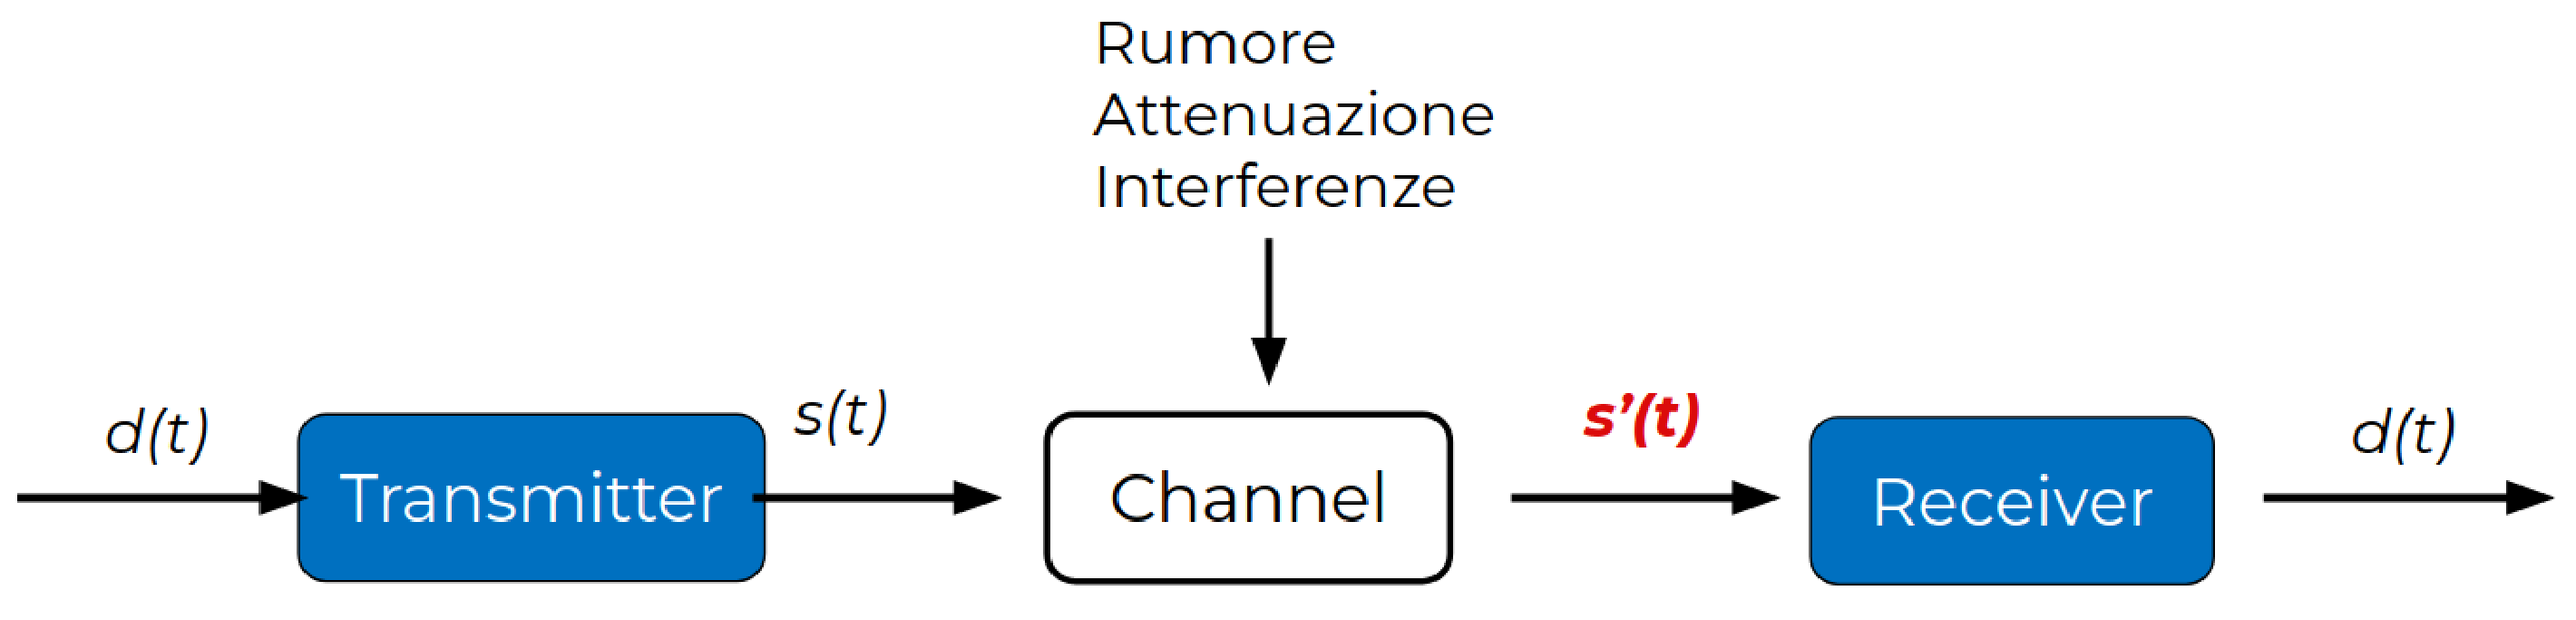
\includegraphics[width=0.95\linewidth]{img/PTT/tr-scheme}
\end{center}

Sono presenti \textbf{dati nel tempo}, questi passano da un \textbf{trasmettitore} il cui ruolo è "tradurre" i dati \textbf{digitali} in un segnale \textbf{analogico}, in quanto deve essere \textbf{trasmesso su un mezzo analogico} (e.g., aria, cavi, ecc.). 

Il segnale attraversa il mezzo e arriva a un ricevitore, il quale decodifica il segnale per tornare ai dati originali. Però, il \textbf{canale non è perfetto} o perfettamente affidabile, è possibile \textbf{introduca}:
\begin{itemize}
	\item Il \textbf{rumore}: in mezzi wireless solitamente non è ignorabile
	
    \item Il ricevitore deve essere in grado di recepire piccole quantità di potenza, in quanto il segnale potrebbe essere \textbf{attenuato}
	
    \item \textbf{Interferenze}, "casuali" dovute alla stessa tecnologia (propagazione del mezzo, ecc.) oppure volontarie (e.g., jamming).
\end{itemize}

Quindi il \textbf{segnale inviato} risulterà \textbf{diverso} dal \textbf{segnale ricevuto}, ma se il segnale viene strutturato correttamente ed è robusto a queste deformazioni il ricevitore sarà in grado di estrapolare ugualmente dati dal segnale "modificato". Quanto è facile ricostruire il segnale dipende da \textbf{quanto} i fenomeni di disturbo hanno \textbf{modificato} il segnale; potrebbe non essere ricostruibile.

Per \textbf{segnale}
\begin{itemize}
	\item \textbf{analogico:} si intende una variazione continua, senza interruzioni o discontinuità
    
	\item \textbf{digitale:} un livello di segnale viene mantenuto costante per un determinato intervallo, con un cambio di livello rapido (quasi istantaneo)
\end{itemize}

Vogliamo passare da una forma d'onda all'altra (trasmettitore e ricevitore fanno questo). 

\subsection{Rappresentazione dei segnali}

\paragraph{Dominio del tempo:} Un segnale può essere visto nel dominio del tempo come un \textbf{segnale periodico sinusoidale}
$$ s(t) = A \sin (2 \pi ft + \phi) $$

Dove: 
\begin{itemize}
	\item \textbf{Ampiezza} $(A)$:	massimo livello o forza del segnale nel tempo (Volt)
	
    \item \textbf{Frequenza} $(f)$: Numero di cicli al secondo (Hz)
	
    \item \textbf{Fase} $(\phi)$: posizione relativa all'interno del periodo
	
    \item \textbf{Periodo} $(T)$: tempo impiegato per un ciclo ($1/f$)
	
    \item \textbf{Lunghezza d'onda} ($\lambda$): distanza occupata da un singolo ciclo: $\lambda = c/f$ oppure $\lambda = T c$ dove $c = 3\cdot 10^8$ m/s
\end{itemize}

La variazione di ampiezza, fase e frequenza vengono usate per codificare le informazioni (e.g., radio AM e FM, modulazione di fase, non usata per le radio).

\paragraph{Dominio delle frequenze:} Possiamo considerare un'onda elettromagnetica guardandola nel tempo, ma anche nel dominio delle frequenze. \textbf{Ogni segnale} (ragionevolmente periodico) \textbf{può essere scomposto da una serie di segnali periodici} (onde seno e coseno) con ampiezza, frequenza e fase differenti: trasformata di Fourier
$$ s(t) = \frac{1}{2} c + \sum_{n=1}^{\infty} a_n \cdot \sin (2 \pi n f t) + \sum_{n=1}^{\infty} b_n \cdot \cos (2 \pi n f t) $$

Dove: 
\begin{itemize}
	\item $f=1/T$: frequenza \textbf{fondamentale} $(n=1)$
	
    \item $a_n, b_n$: \textbf{ampiezza} delle \textbf{singole componenti}, dette armoniche
	
    \item $c$: costante che rappresenta il \textbf{valore medio} del \textbf{segnale}
\end{itemize}

Possiamo \textbf{scomporre} un segnale in \textbf{diverse armoniche}, ognuna con il suo "contributo" rispetto al segnale originale. Questa è la serie di Fourier discreta. Discreta perché in un calcolatore saranno un numero finito di frequenze, si può avere anche la versione con integrali, nel continuo.

Insomma, serve per passare da un dominio all'altro.

\paragraph{Cosa ci interessa:} Dal punto di vista di un ricevitore, il quale riceverà tali segnali, ci interessa capire \textbf{com'è composta l'onda} a partire \textbf{da un'osservazione nel tempo} di quest'onda. Come faccio a \textbf{risalire alle componenti} a partire da un'osservazione nel tempo della forma d'onda? 

Le domande sono: 
\begin{enumerate}
	\item Come si fa a \textbf{determinare} le \textbf{ampiezze} di ciascuna componente
	
    \item Con quale \textbf{frequenza campionare il segnale}? Il mondo digitale è discreto per definizione, in che punti della curva bisogna "leggere" per poter ricostruire l'onda in maniera precisa
\end{enumerate}

\paragraph{Teorema del campionamento di Shannon:} La \textbf{frequenza di campionamento} deve essere almeno il \textbf{doppio della frequenza massima del segnale} in ingresso.
\label{par:shannon}

Sapendo la frequenza massima (ricevitore e trasmettitore ne sono a conoscenza), bisogna campionare ad almeno il doppio per evitare perdita di dati.

\paragraph{Passaggi di dominio:} Per passare da un dominio all'altro si hanno due algoritmi:
\begin{itemize}
	\item \textbf{Fast Fourier Transform FFT:} da tempo a frequenze, a partire dalla forma d'onda nel tempo restituisce le componenti
	
    \item \textbf{Inverse Fast Fourier Transform IFFT:} da frequenze a tempo, partendo dalle componenti restituisce la forma d'onda
\end{itemize}

Con "\textit{componenti}" si intende i coefficienti $a_n$ e $b_n$ viste nella serie di Fourier. Questi algoritmi sono semplici, vengono implementati tramite hardware nei dispositivi, i quali devono effettuarle costantemente.

Assegnando dei bit al fingerprint di una forma d'onda (valori della trasformata), posso creare una \textbf{lookup table} per trovare il "significato" di una forma d'onda a partire dalla sua trasformata. In generale: osservo l'onda, trasformata, lookup su una tabella per avere il significato.

Nel dominio delle frequenze: quando \textbf{tutte le frequenze} sono \textbf{multipli interi di una frequenza base}:
\begin{itemize}
	\item $f=$ \textbf{frequenza fondamentale}
    
	\item $kf =$ \textbf{armonica} ($k>1$)
\end{itemize} 

\paragraph{Periodo:} Il periodo di $s(t)$ è il periodo della frequenza fondamentale $(T = 1/f)$.

\paragraph{Spettro:} Lo spettro del segnale è il range di frequenze che lo contiene (da dove a dove vanno le frequenza).

\paragraph{Banda:} Absolute bandwidth è l'ampiezza dello spettro ("larghezza" dello spettro).

\subsection{Relazione tra Bandwidth e Data Rate}

Volendo trasmettere un'onda quadra come \textbf{composizione finita di onde sinusoidali}. Esempio:
\begin{center}
	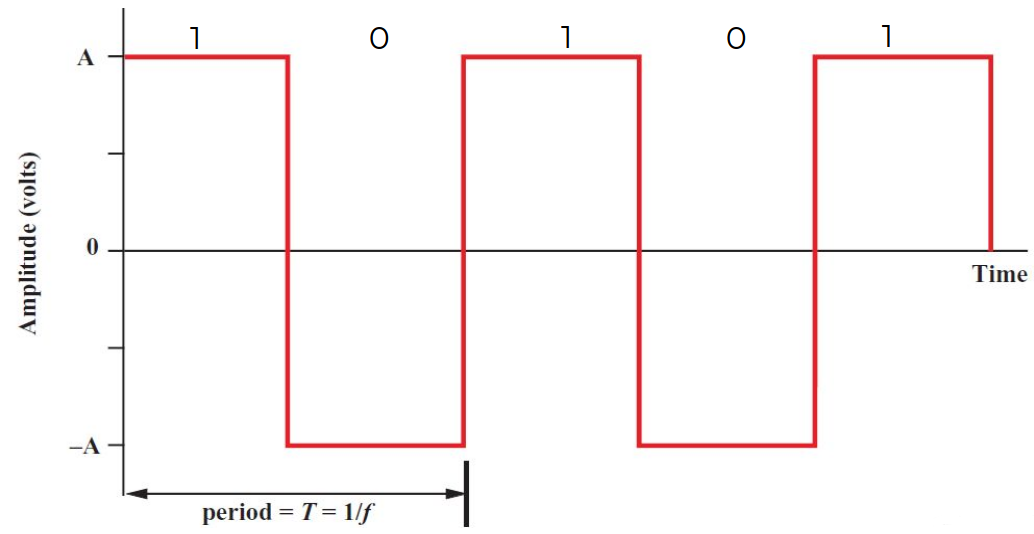
\includegraphics[width=0.7\linewidth]{img/PTT/quadra1}
\end{center}

Trasmettiamo 2 bit per ogni periodo, ovvero un data rate di 2 bit. Possiamo avere una \textbf{sommatoria} infinita di onde \textbf{sinusoidali}: 
$$ s(t) = A \cdot \frac{4}{\pi} \cdot \sum_{k \text{ odd}, k=1}^{\infty} \frac{\sin (2 \pi kft)}{k} $$

Ma questo \textit{richiederebbe una banda infinita} (difficile) quindi possiamo \textbf{ridurre lo spettro} per ottenere un'\textbf{approssimazione}: 
\begin{center}
	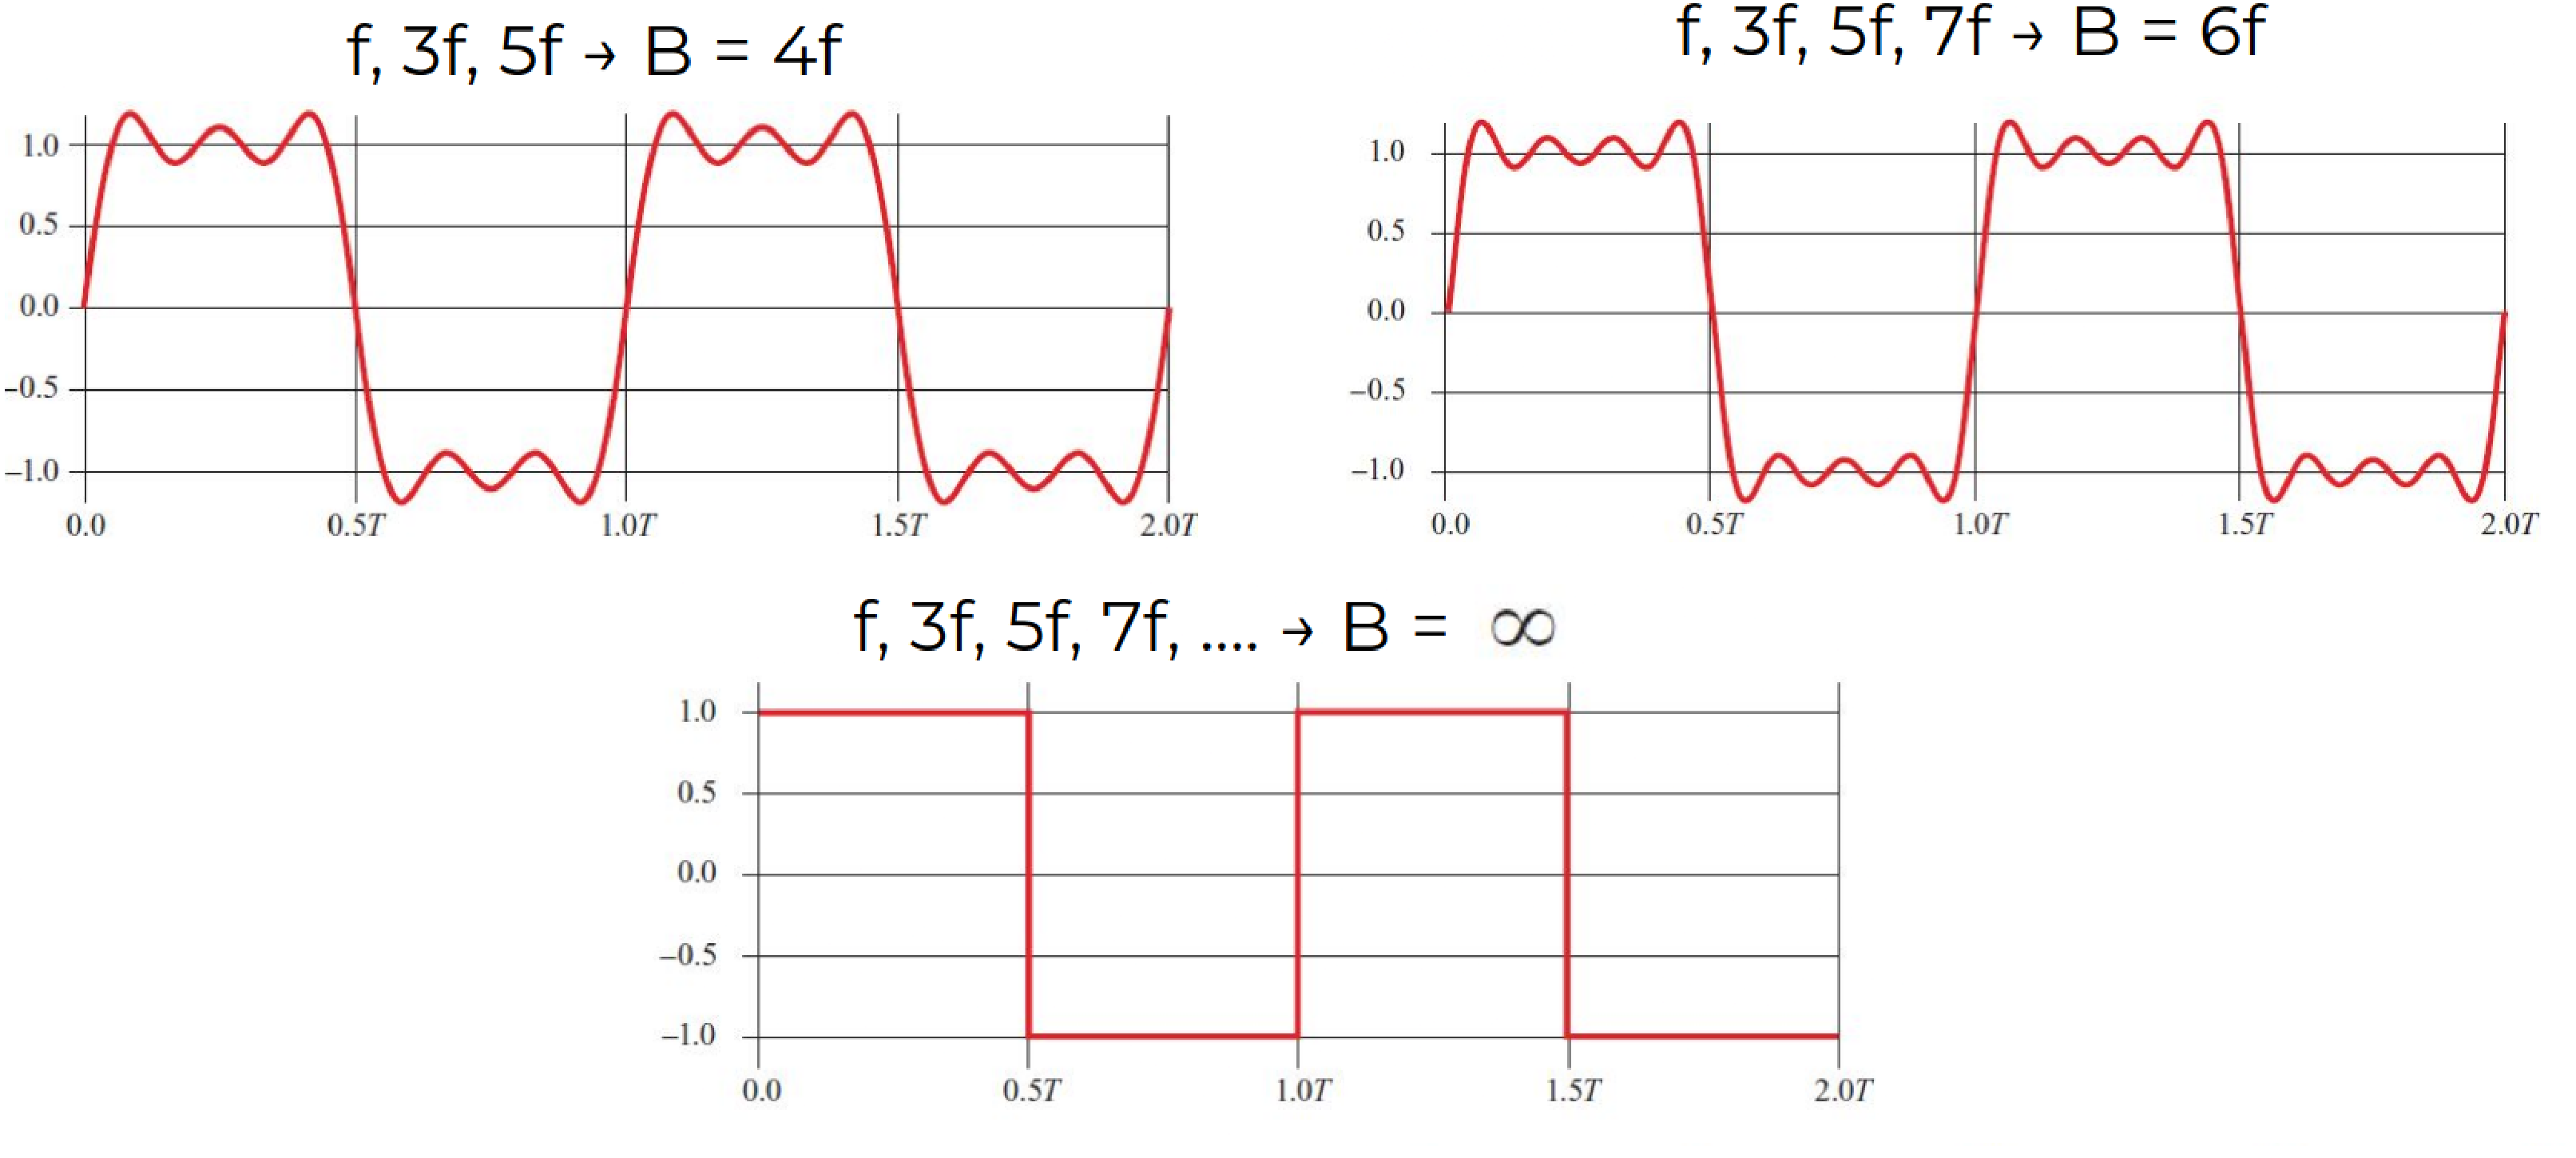
\includegraphics[width=\linewidth]{img/PTT/fourier1m}
\end{center}

Nel primo esempio una banda di $4f$ che va da $f$ a $5f$, nel secondo aumentiamo la banda a $6f$, migliorando l'approssimazione. Facendo tendere a infinito si ottiene l'onda originale.

Con una certa banda, \textbf{quanti dati possiamo trasmettere?} Esempio: 
\begin{center}
	\begin{tabular}{| c | c | c |}
		\hline
		Freq. fondamentale $(f)$ & 1 MHz & 2 MHz \\
		\hline
		Spettro & 1 Mhz - 5 Mhz & 2 Mhz - 10 Mhz \\
		\hline
		Periodo (T) & 1 $\mu$s & 0.5 $\mu$s \\
		\hline 
		Durata di 1 bit & 0.5 $\mu$s & 0.25 $\mu$s \\
		\hline
		Bandwidth (B) & 4 Mhz ($5f - f$) & 8 Mhz ($2(5f - f)$) \\
		\hline
		Data rate (bps) & 2 Mbps (2 bit/$\mu$s) & 4 Mbps (4 bit/$\mu$s) \\ 
		\hline
	\end{tabular}
\end{center}
Con il doppio della banda viene raddoppiato il data rate.

\paragraph{Capacità del canale:} Quanti bit si possono trasmettere sul canale senza perdere informazioni?
\begin{itemize}
	\item \textbf{Channel capacity:} massimo bit rate alla quale è possibile trasmettere dati su un canale di comunicazione in determinate condizioni

	\item \textbf{Noise:} segnale NON voluto che si combina al segnale trasmesso, distorcendolo

	\item \textbf{Error rate:} tasso di errore (bit error rate), quante volte viene modificato involontariamente il segnale
\end{itemize}

Come possiamo trasmettere la \textbf{stessa quantità di informazioni senza usare più banda}? La soluzione è \textbf{ridurre il numero di armoniche}, semplificando la forma d'onda, di conseguenza peggiorando l'approssimazione. Questo si può fare finché l'onda non è un'approssimazione "troppo approssimata" (deve rimanere distinguibile).

\paragraph{Considerazioni:} Vogliamo trasmettere una banda infinita con banda finita, ma una banda minore porta a distorsione maggiore. Una soluzione potrebbe essere scegliere la banda finita più ampia; sarebbe fattibile ma ci sono costi economici (i.e., la banda non è gratis) e il dispositivo deve essere in grado di gestirla. Inoltre può creare rumore aggiuntivo.

\subsubsection{Teorema di Nyquist sulla banda}

Dato un canale noise-free (ideale) la bandwidth limita il data-rate. Il \textbf{limite della quantità di informazioni} (misurata in bit/secondo e multipli) è limitato da due volte la banda
$$ C = 2B $$
per \textbf{segnali binari} (2 livelli di voltaggio). Per \textbf{segnali multilivello}, codificare i dati su più livelli di segnale
$$ C = 2B \log_2 M $$
dove $M$ è il numero di livelli.

La \textbf{capacità del canale aumenta con il numero di possibili livelli} in cui codificare il segnale, modificando uno dei parametri (ampiezza, frequenza, fase). Il numero di livelli di segnale aumenta il numero di bit che si possono trasmettere con ogni trasmissione: con 2 valori trasmettiamo 1 bit, con 8 possibili valori possiamo trasmettere 3 bit alla volta. 

Questa è la capacità possibile solo se in assenza di rumore, ovvero il massimo possibile. Tenendo il considerazione il rumore la capacità (ovviamene) si abbassa.

Esempio di effetto del rumore sul segnale trasmesso: 
\begin{center}
	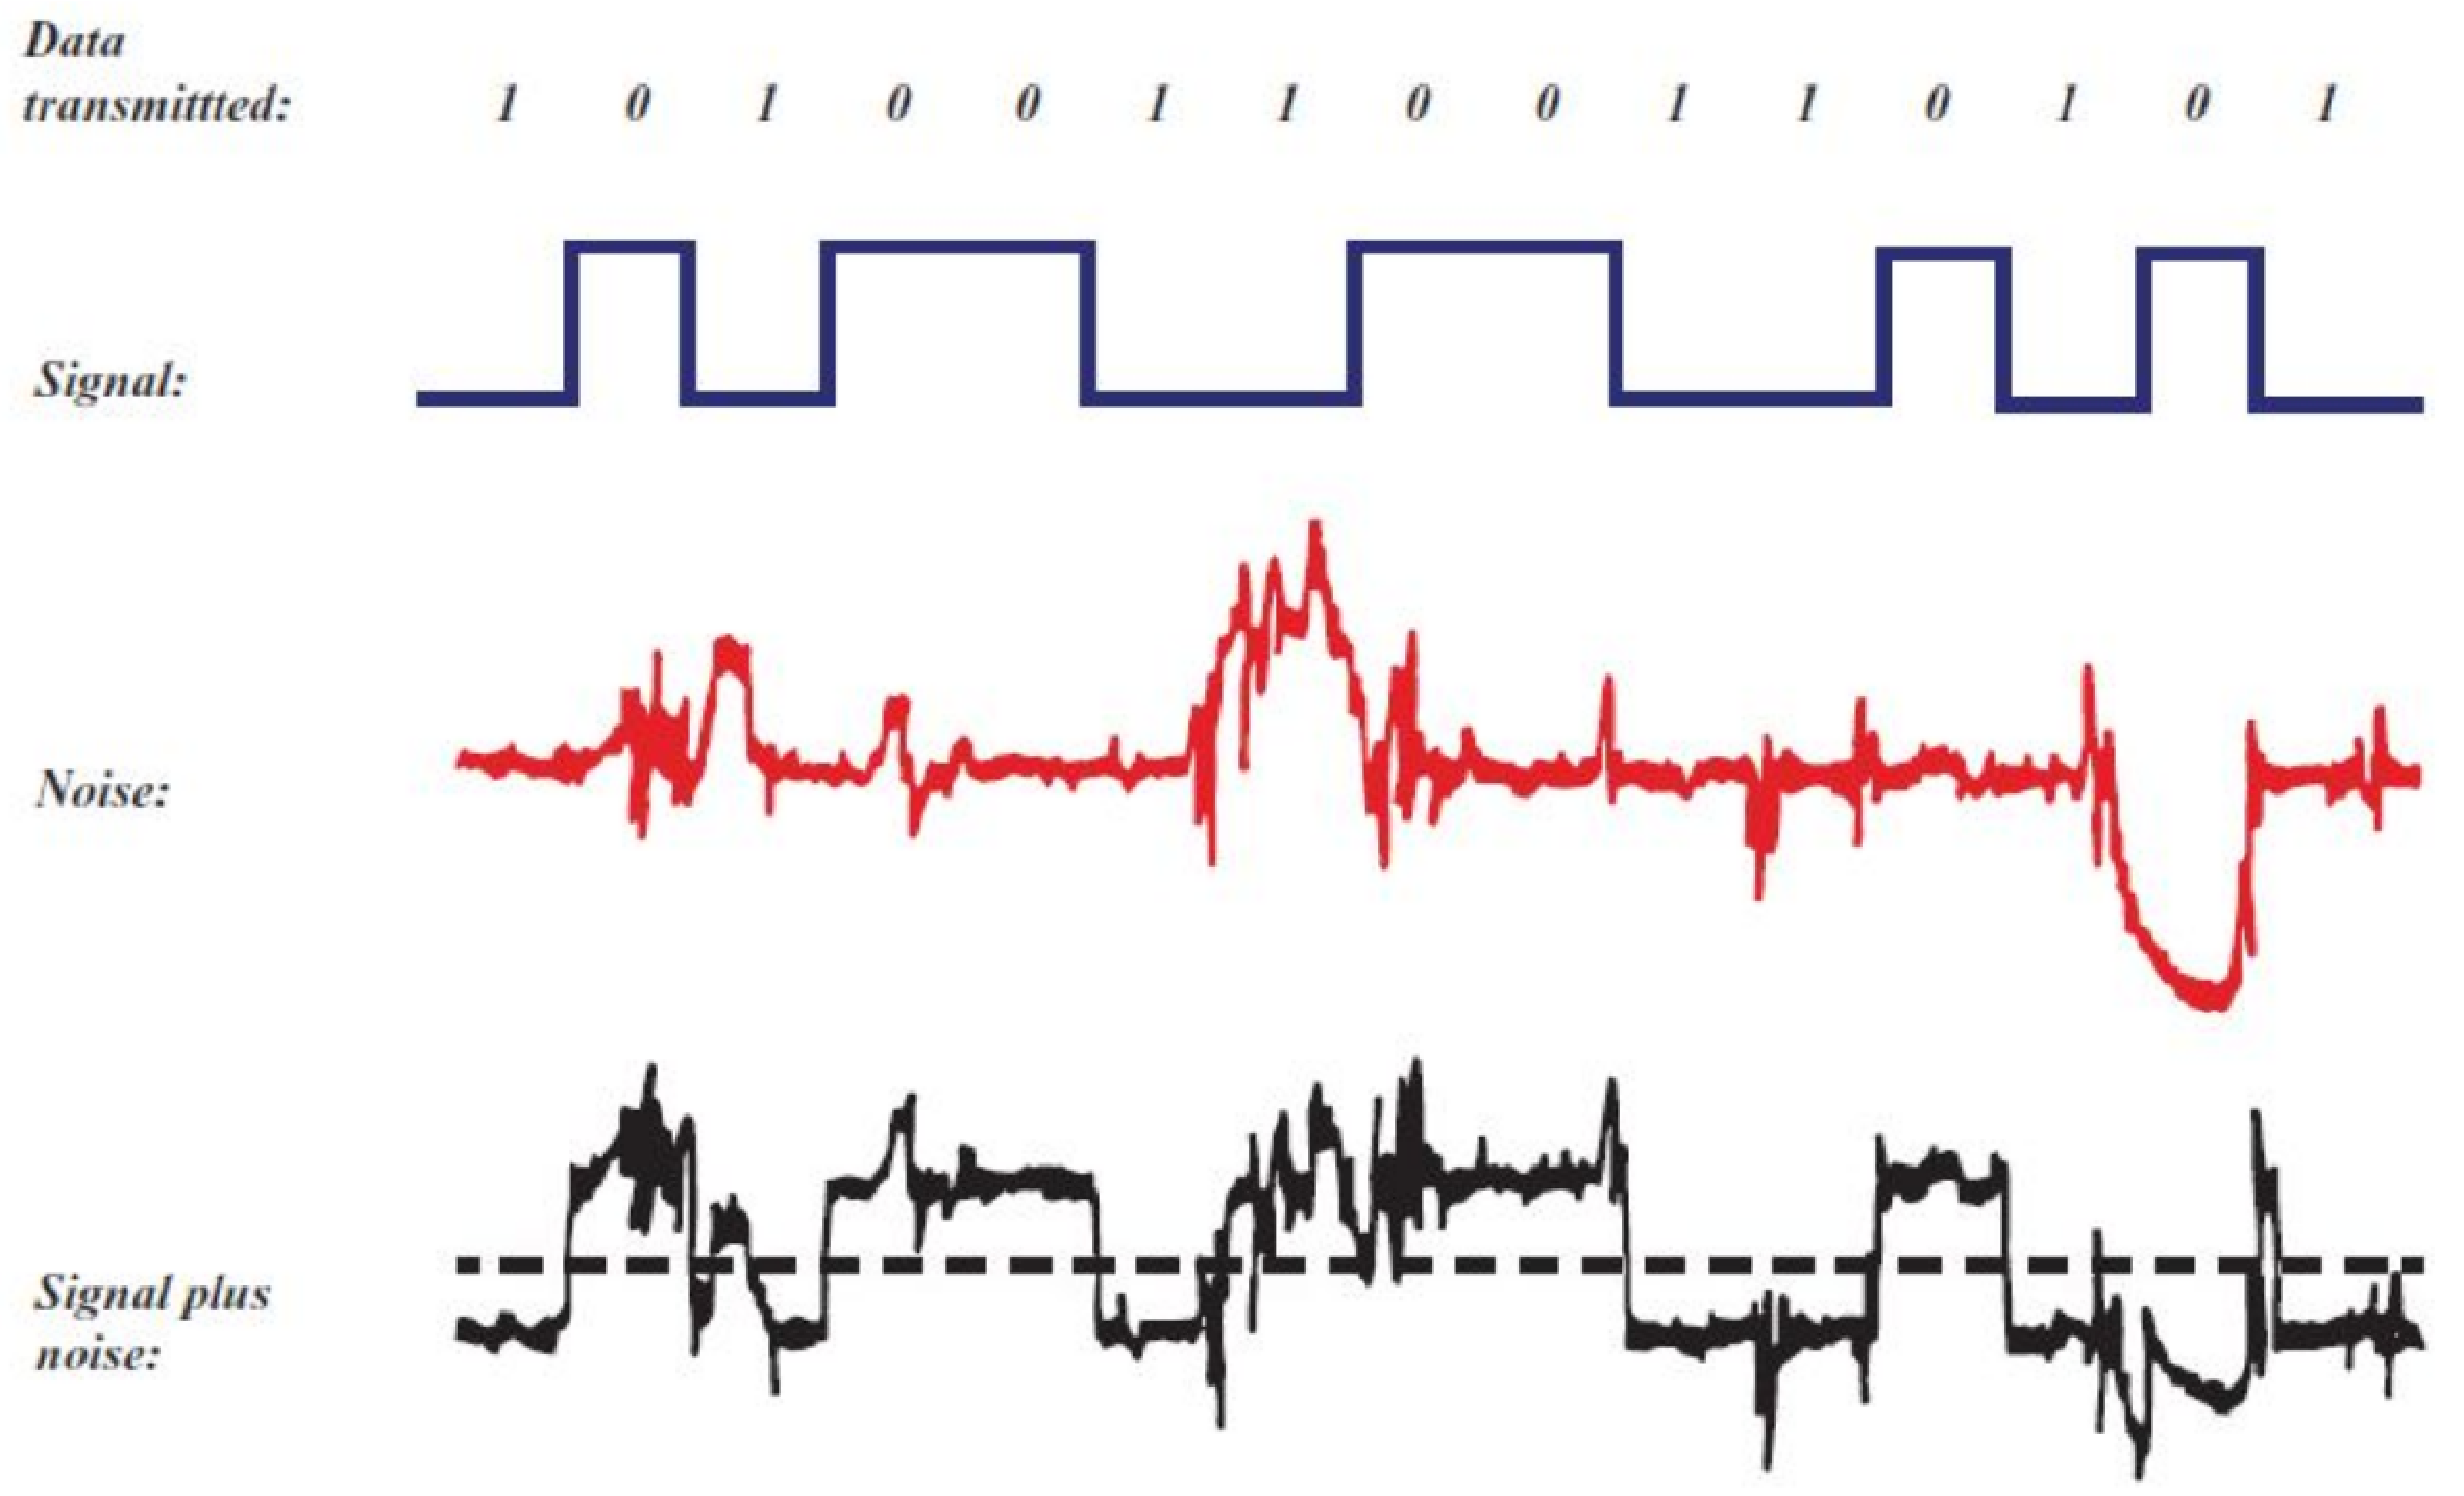
\includegraphics[width=\linewidth]{img/PTT/errors1}
\end{center}

Considerando il profilo temporaneo del rumore, il ricevitore capta un segnale (anche molto) diverso, affetto da modifiche su cui non si può avere controllo, indipendenti da ricevitore e trasmettitore.

% End L1

\paragraph{Tipi di rumore:}
\begin{itemize}
	\item \textbf{Thermal noise}: rumore di base dovuto all'agitazione delle molecole, un rumore bianco costante su tutta la banda

	\item \textbf{Intermodulation noise}: determinato dal fatto che ci sono dei problemi tra le diverse modulazioni, ci si "accavalla" nel trasmettere le informazioni

	\item \textbf{Cross talk}: cavi vicini che alterano il segnale l'uno dell'altro, tramite radiazioni elettromagnetico

	\item \textbf{Impulse noise}: impulso elettromagnetico intenso di durata limitata che attraverso il mezzo e distrugge temporaneamente il segnale
\end{itemize}

\subsubsection{Decibel}
Il decibel è un'\textbf{unità di misura del rapporto di potenze}, in \textbf{scala logaritmica}
$$ \left(\frac{P_1}{P_2}\right)_{dB} = 10 \cdot \log_{10} \left(\frac{P_1}{P_2}\right) $$ 
$\pm 3$ corrispondono al doppio/metà.

\paragraph{Decibel-Milliwatt:} Un decibel ma con la \textbf{potenza al denominatore fissata} ad $1mW$
$$ P_{dBm} = \frac{P}{1mW} $$

Generalmente una Wireless-LAN (WiFi 802.11) usa $100mW$, quindi $20dBm$, mentre, una trasmissione cellulare usa $500mW$, quindi $27dBm$ (ricorda di mettere dopo il $10 \log_{10}$). In generale, una lettera dopo $dB$ indica una potenza fissata al denominatore.

\subsubsection{Rapporto segnale rumore SNR}

Dobbiamo essere un grado di \textbf{quantificare il rumore} su un canale, quindi l'impatto sul rumore della trasmissione.
$$  (SNR)_{dB} = 10 \log_{10} \frac{\text{signal power}}{\text{noise power}} $$

Misurato in decibel (rapporto tra due potenze), tanto più il rapporto è alto, tanto più il segnale si distingue dal rumore.

\subsubsection{Shannon Capacity Formula}
Nyquist descrive la capacità del canale nel caso di assenza di rumore, Shannon dice che la \textbf{capacità dipende} non solo dalla capacità di codificare livelli ma \textbf{anche dal SNR}
$$ C = B \log_2 (1 + SNR) $$

Quindi la \textit{capacità è direttamente proporzionale al SNR}. Questo valore è puramente teorico e \textbf{considera solo il thermal noise}, ma fornisce una \textbf{massima teorica per trasmettere informazioni senza errori} su un canale. La teoria della trasmissione di Shannon ha come assioma una trasmissione senza errori.

In una determinata condizione di rumore (SNR) possiamo aumentare il data rate in due modi:
\begin{enumerate}
	\item Aumentando la bandwidth ($B$), ma il rumore termico aumenta con la larghezza della banda
	
    \item Aumentando la potenza del segnale trasmesso (quindi aumentando il valore del SNR), ma un aumento della potenza porta ad aumentare intermodulation e crosstalk noise (aumenta il campo elettromagnetico)
\end{enumerate}

Posso aumentare SNR o $B$ ed in entrambi i casi l'aumento viene "bilanciato" da un aumento del rumore.

\paragraph{Esempio:} Supponiamo di avere a disposizione uno spettro tra $3 MHz$ e $4 MHz$ e $SNR_{dB}=24dB$:
\begin{align*}
	B & = 4Mhz - 3Mhz = 1 Mhz \\
	SNR_{dB} & = 24dB = 10 \log_{10} (SNR) \\
	\implies SNR & = 251
\end{align*}

Il valore di $SNR$ significa che il segnale è circa 251 volte superiore al rumore. Ora possiamo calcolare la capacità secondo Shannon:
$$ C = 10^6 \cdot \log_2 (1 + 251) \approx 10^6 \cdot 8 = 8 Mbps $$

E da questa possiamo trovare quanti livelli di segnale servono per ottenere $8Mbps$, tramite la formula della capacità secondo Nyquist:
$$\begin{array}{c c r c l}
	C = 2B \log_2 (M) & \implies & 8 \cdot 10^6 &=& 2 \cdot 10^6 \cdot \log_2(M) \\
	& \implies & 4 &=& \log_2 (M)  \\
	& \implies & M &=& 16 \\
\end{array}$$

Più di 16 sarebbe inutile perché trasmettendo un numero maggiore di livelli non possiamo superare la capacità teorica detta da Shannon. La capacità dipende dalla condizione del canale e dal numero di livelli.

\subsection{Multiplexing}

L'idea è quella di un \textbf{collegamento che può trasportare più canali}. Solitamente la capacità di un mezzo è superiore della capacità richiesta da una singola trasmissione: si vuole un modo di trasportare più segnali sullo stesso collegamento.

\subsubsection{Frequency Division Multiplexing FDM}

Avendo una banda "larga", la si può dividere in "slot" per ottenere sotto-bande, ognuna con una comunicazione diversa. Si sfrutta il fatto che ogni segnale da trasmettere richiede una banda minore di quella disponibile. Creiamo $n$ canali paralleli all'interno della banda.

\begin{center}
	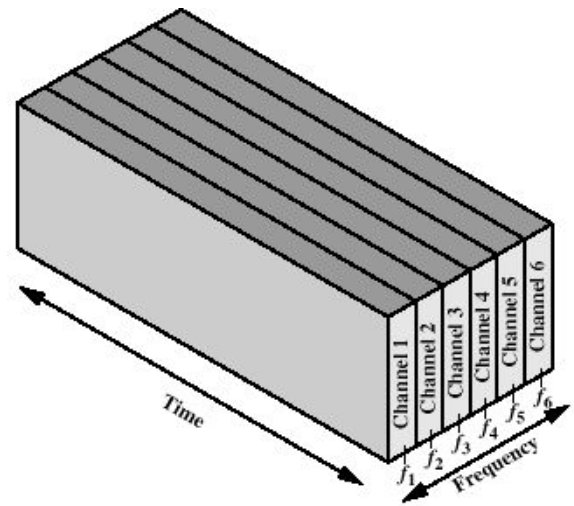
\includegraphics[width=0.4\linewidth]{img/PTT/fdm1}
\end{center}

\subsubsection{Time division Multiplexing TDM}
Se la banda è "piccola", ma il data rate è molto superiore a quello richiesto da una singola trasmissione, si possono creare $n$ slot di tempo ciclici, alternati uno dopo l'altro.
\begin{center}
	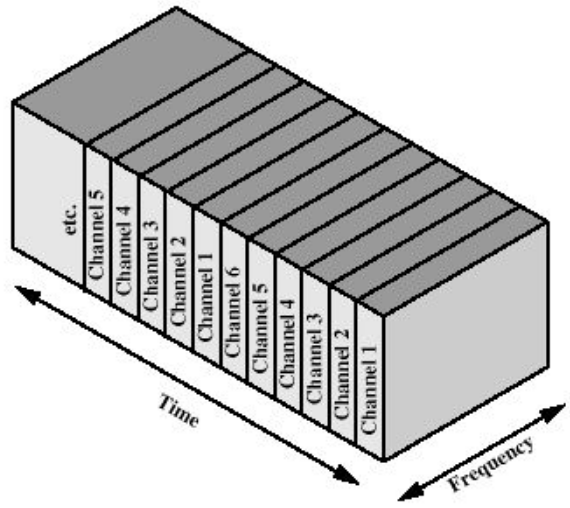
\includegraphics[width=0.4\linewidth]{img/PTT/tdm1}
\end{center}